%--------------------------------------------------------------------------------------------------
% 
\chapter{Introduction}
\label{ch:introduction}
%--------------------------------------------------------------------------------------------------

\epigraph{In theory, theory and practice are the same. In practice, they are not.}{\textit{Albert Einstein}}

% V uvodu magistrskega dela oz. doktorske disertacije mora biti jasno povzeta teza iz prijave teme magistrskega dela oz. doktorske disertacije. Dosežki so praviloma predstavljeni strokovni javnosti. Glavno besedilo magistrskega dela oz. doktorske disertacije se lahko nadomesti z objavami (oziroma z deli, sprejetimi v objavo) v uglednih mednarodnih revijah.

% To pomeni, da praviloma poglavja v disertaciji ostanejo enaka, le da namesto poglavij, v katerih bi praviloma dokazovali posamezno hipotezo, zamenjate s članki (1 članek = 1 poglavje), v uvodu posameznega poglavja s člankoma pa navedete opis znanstvene metode ter vaš prispevek k posamezni objavi.

With the growth of the number of smart sensors, we are increasingly able to access vast amounts of data that can be used to improve knowledge about observed systems. 
This data has high frequency and is often updated in (almost) real time.
Because of this, Internet of Things (IoT) has also changed the focus in machine learning from offline analysis (batch) to real-time (online) prediction and analysis. 

To achieve the full analytical potential of the streaming data from the internet of things, the interconnection of various data sources is needed.
By definition, those sources are heterogeneous and their integration is not a trivial task.
A common approach to exploit streaming sensor data potential is to use machine learning techniques for predictive analytics in a way that is agnostic to the domain knowledge.
Such an approach can be easily integrated in various use cases.

In the dissertation we consider a methodology for development and deployment of real-world machine learning models, that solve problems such as: predicting energy consumption on smart-grid or demand of potable water in a water distribution network in the next days, predicting groundwater and surface water levels at various spatial points, predicting energy demand of an electrical train, etc.

The purpose of the dissertation is to develop a generic pre-processing framework for heterogeneous data streams and test its modeling capabilities in real-world scenarios. 
The core of the framework is a real-time data fusion component, which is able to integrate several heterogeneous real-world data sources (streams or static) into a descriptive feature vector. 
The framework is based on the lambda architecture approach, which divides processing into two pillars: speed (real-time) and batch. 
We propose a modeling workflow, where the model is developed in a batch setting (including automated feature selection) and then pushed into the deployment and chained with autonomous data cleaning, feature engineering and heterogeneous streams data fusion. 

We base our work on the Big Data lambda architecture (see Figure \ref{fig:the_big_picture}), building on 2 main pillars (batch: for offline data analysis – and speed: for online analysis and deployment of the real-time models) \cite{kenda:2022:water-framework}.
We propose a workflow for development and deployment of machine learning models, that extends initial lambda architecture proposal.
Our main innovation is the extension of the speed pillar, where we overcome the limits of simple event detection and processing.
We introduce autonomous online data fusion of heterogeneous data sources \cite{kenda:2019:fusion}, which supports either incremental models (online training and inference) or batch model inference and training data generation.
We propose also an autonomous data cleaning methodology based on Kalman filter for sensor data cleaning \cite{kenda:2018:autonomous}.
In the batch pillar, the tools have been developed in depth in the past and several industry-standard tools already exists (from data storage to data manipulation and model development).
In the batch pillar we propose a novel feature selection methodology (FASTENER), based on a genetic algorithm \cite{koprivec:2020:fastener}.
The methodology is able to select a subset of relevant features faster than competing algorithms and offer fast model development even with large datasets.
Several offline and online modeling techniques dealing with time-series prediction and anomaly detection (\cite{kenda:2022:water-framework, kenda:2015:modelling, kenda:2015:modelling2, petkovsek:2021:anomaly, costa:2021:entropy}), both batch and incremental, were tested in the scope of the proposed framework.

\begin{figure}
    \centering
    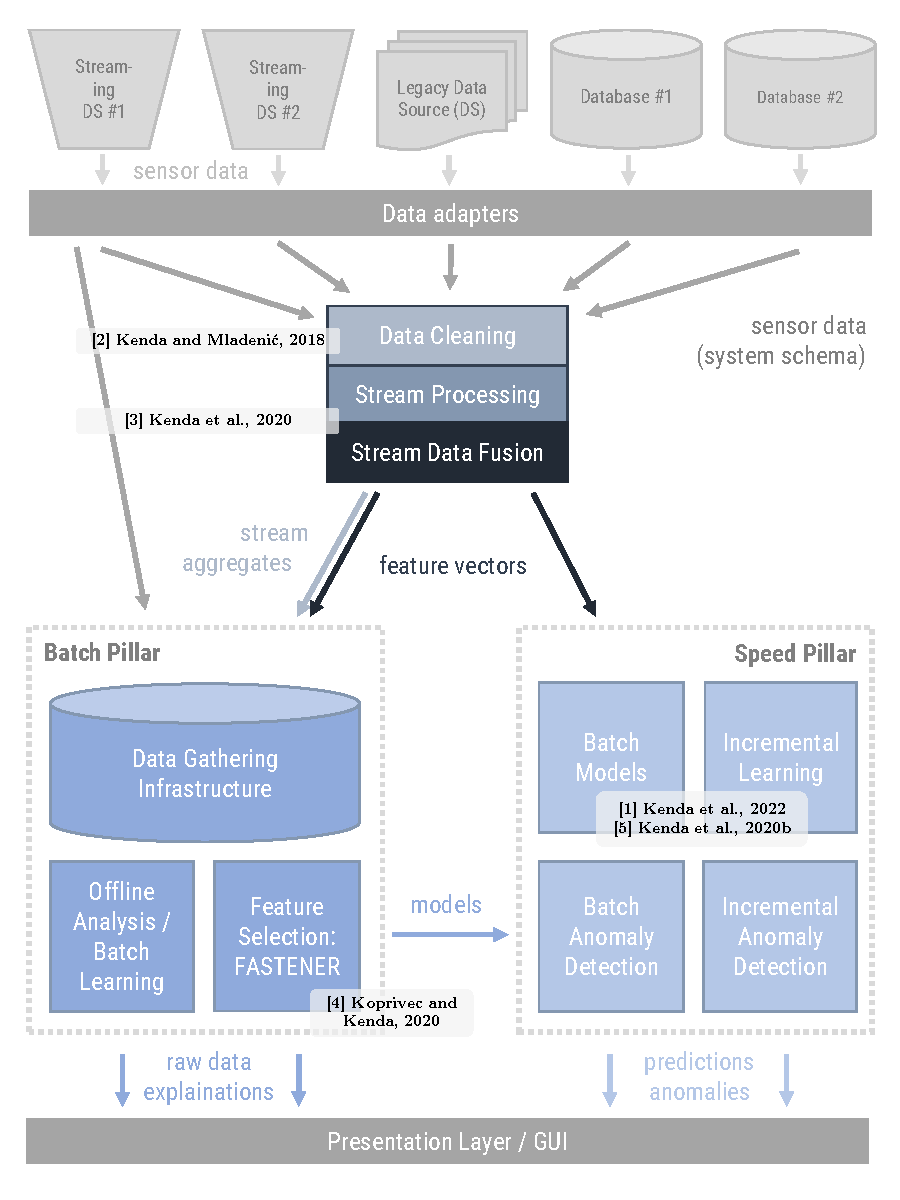
\includegraphics[width=15cm]{figures/the_big_picture_2023a.pdf}
    \caption{Lambda architecture for processing Big Data with references to journal papers describing particular components. Paper \cite{kenda:2022:water-framework} also describes the overall architecture of the system.}
    \label{fig:the_big_picture}
\end{figure}

\section{Motivation}

The scientific community has been discussing the rising amount of data originating from the internet of things (IoT) for more than a decade. The IoT reached the mass market in early 2014 and its ubiquitous influence and challenges are still permeating the scientific literature. 
The field of big data processing has improved drastically and a plethora of solutions for various IoT problems have reached their production stage.

The volume of the data keeps rising and as the technology is penetrating new markets (e.g., water management), new challenges are put in front of the industry and academia. 
The need for efficient and accurate analysis of these data is still an issue. 
Stream processing has been established as a potential answer to the analysis of big data and incremental learning has been rediscovered to answer some of the challenges (like concept drift or learning efficiency). 
While the field of incremental learning has matured through the last decade and a wide variety of algorithms have been described, tested and implemented in various software libraries, the applications of methodologies from a laboratory to the real world have been scarce.

Throughout our work in various applications within the environmental domain, water management, traffic, energy efficiency and smart grid modeling, we have (among others) identified the following shortcomings: most of the scientific work on incremental learning has taken place inside the lab, emulating unreal (ideal) conditions, which are rarely encountered in the real world; mostly this remark applies to the data availability and data preparation step (including data fusion and generation of machine-learning-ready rich data streams).

The ongoing lack of on-line data pre-processing techniques (\cite{kolajo:2019:big, bahri:2021:data}) reduces the possibility of using streaming and also hybrid approaches in real world scenarios, where data pre-processing is done on-line and prediction models are implemented using traditional machine learning (ML) approaches. 
McKinsey \cite{manyika:2015:unlocking} has established that up to $40\%$ of the data value emerging from the IoT is hidden within the synergy effects of different systems. 
With the exception of the IoT Streaming Data Integration (ISDI) framework \cite{tu:2020:isdi} which solves time alignment issues of data integration, a generic methodology for generation of feature vectors for machine learning approaches in the IoT scenario does not yet exist and this work aims to fill this gap.
Other proposed solutions (\cite{zhang:2019:advanced, wu:2018:sensor, zhou:2018:multimodal, wu:2019:fusion, akbar:2018:real}) are able to solve application problems, however they lack the functionality to be implemented in a general scenario.

The framework, proposed in the dissertation, offers a complete streaming methodology for building rich feature vectors, describing important process characteristics (or features), suitable for traditional or incremental machine learning algorithms. 
Within the dedicated big data framework, the proposed methodology is able to merge data from a set of heterogeneous streaming data sources (i.e., from the IoT, weather forecasts and data about human behavior) in a real-world setting and enables machine learning models to yield more accurate and thus more useful results in real time.

\section{Aims and Hypotheses}

\noindent The thesis has two main hypotheses that will be addressed and experimentally tested.

\begin{itemize}
    \item \textbf{Hypothesis 1}: \textit{Including multiple relevant data-sources improves the overall models’ performance in real-time predictive time-series analytics.} 
    
    \textbf{Prior state of the art:}
    A generic incremental framework for data fusion in the incremental setting has not been available before the work accomplished for \cite{kenda:2019:fusion}.
    Majority of the incremental learning literature assumes artificial modeling scenarios, where all the data is available immediately (no delays, no missing/wrong data).
    It is a well known fact that usage of several contextual data sources adds to the overal information gain and therefore improves the models' performance, which has been tested in several settings, mostly batch (offline).
    
    \textbf{Aim:} 
    Our goal is to create a formal definition of data fusion of heterogeneous streaming data sources, as well as autonomous methodologies and prototypes for online data cleaning (based on Kalman filter), fusion and enrichment of heterogeneous data streams. 
    With the vast number of derived time series from the original data, our goal is to develop a novel algorithm for feature selection based on information theory and multi objective optimization approach, which would enable efficient definition of feature vectors.
    
    \item \textbf{Hypothesis 2}: \textit{Unified big data architecture including autonomous data cleaning and heterogeneous source data fusion is suitable for different real-world scenarios (IoT, earth observation, energy grids).}

    \textbf{Prior state of the art:}
    Several proposals for the Big Data architectures have been proposed.
    The lambda architecture already distinguishes between two main pillars - batch (for offline processing) and speed (for online processing).
    However, in all the definitions, the speed pillar is only composed of (complex) event processing and does not include other analytical functionalities.
    Most of the research dealing with contextual data is performed offline, the dedicated systems are run in batched mode or the online fusion is suitable only for a specific application.
    
    \textbf{Aim:}
    Our goal is to propose an extension to big data lambda architecture for hybrid model development and deployment that will also include analytical capabilities (such as predictive analytics and anomaly detection) in the speed pillar as well as means for pushing the trained model (or incremental model definitions) from batch to speed pilar (house architecture).
    Our aim is also to introduce and test the feasibility of incremental learning in the field of water management and earth observation.
    Finally, we aim to evaluate the proposed architecture and methods in several real-world scenarios from the energy management, water management, smart cities, transport energy management and earth observation domains.
    
\end{itemize}

\section{Scientific Contributions}

Main scientific contributions of the dissertation are as follows:

\begin{itemize}    
    \item \textbf{SC1 - Data cleaning and fusion, feature generation (enrichment) and selection}: Development of autonomous methodologies for online data cleaning (based on Kalman filter), fusion and enrichment of heterogeneous data streams. Development of a novel algorithm for feature selection based on information theory and multi objective optimization approach.
    \item \textbf{SC2 - Architecture}: Development of an extension of lambda (big data) architecture for hybrid ML model development (batch) and deployment (in real-time).
    \item \textbf{SC3 - Evaluation in real-world scenarios}: Evaluation of the proposed architecture and methods in several real-world scenarios from the energy management, water management, smart cities, transport energy management and earth observation domains.
\end{itemize}

\section{Organisation of the Thesis}

Thesis begins with an introduction, motivation and an overview of the aims, hypotheses and scientific contributions.
Along the published journal papers, the latter are presented in Figure \ref{fig:the_big_picture}.

Chapters \ref{ch:data-cleaning} through \ref{ch:big_data_framework} present 5 papers, published in peer review journals.
Each chapter gives a short introduction to the presented paper and then presents it in the same format as published in the journal.
Chapter \ref{ch:data-cleaning} is dedicated to the first step in the overall picture (see Figure \ref{fig:the_big_picture}) - data cleaning [\textbf{SC1}]. The chapter presents a paper titled \textit{Autonomous Sensor Data
Cleaning in a Stream Mining Setting}~\cite{kenda:2018:autonomous}.
In Chapter \ref{ch:data-fusion} we proceed with the introduction of the online heterogeneous data fusion tailored for machine learning applications [\textbf{SC1}].
The paper title \textit{Streaming data fusion for the internet of things}~\cite{kenda:2019:fusion} represents the the cornerstone of the thesis.
In order to efficiently use data fusion, an efficient feature selection is needed.
A novel feature selection algorithm called FASTENER, based on genetic algorithms and multi-objective optimization approach, is presented in Chapter~\ref{ch:feature-selection} [\textbf{SC1}] alongside the paper titled \textit{FASTENER feature selection for inference from earth observation data}~\cite{koprivec:2020:fastener}.
Next, in Chapter \ref{ch:big_data_framework} we present an implementation of the framework based on architecture and components presented in this thesis [\textbf{SC2}] as well as the final piece in the mosaic, the usage of incremental learning techniques in the platform.
The framework is decribed in depth in the paper titled \textit{Computer Architectures for Incremental Learning in Water Management}~\cite{kenda:2022:water-framework}, whereas incremental learning techniques have been tested in \textit{Usage of statistical modeling techniques in surface and groundwater level prediction}~\cite{kenda:2020:water-modeling}.

Evaluation of the methodologies in the real-world scenarios [\textbf{SC3}] is given in each of the presented papers from Chapter \ref{ch:data-cleaning} trough \ref{ch:big_data_framework}.

Chapter \ref{ch:conclusion} concludes the thesis by looking back at the main scientific contributions and clearly stating objectives and directions for future work and research on the topic of pre-processing of heterogeneous data streams for Internet of Things applications.
